\documentclass[conference]{IEEEtran}

\IEEEoverridecommandlockouts

\usepackage[utf8]{inputenc}
\usepackage[T1]{fontenc}

\usepackage{cite}

\ifCLASSINFOpdf
  \usepackage[pdftex]{graphicx}

\else

\fi

\usepackage[cmex10]{amsmath}

\usepackage{multirow}
\usepackage{array}
\usepackage[lofdepth,lotdepth]{subfig}
\usepackage{color}
\usepackage{tabto}

\usepackage{amssymb}
\usepackage{booktabs}
\usepackage{multirow}
\usepackage{rotating}
\usepackage{amsmath}
\usepackage{algorithm}
\usepackage{algpseudocode}
\usepackage{lineno,hyperref}
\usepackage{graphicx}
\usepackage{pdflscape}
\usepackage[none]{hyphenat}

\begin{document}

\IEEEpubid{\makebox[\columnwidth]{\hfill} \hspace{\columnsep}\makebox[\columnwidth]{}}

\title{Kırmızı Şarap Kalitesinin Makine Öğrenmesi Kullanılarak Tahmin Edilmesi
\\
\*

Predicting Red Wine Quality Using Machine Learning
}
\author{
	
\IEEEauthorblockN{Mehtap ÖKLÜ}
\IEEEauthorblockA{Bilgisayar Mühendisliği\\
	17110131052\\
	Kahramanmaraş Sütçü İmam Üniversitesi\\
	Kahramanmaraş, Türkiye\\
	mehtap\_oklu\_06@hotmail.com
	}
\and
\IEEEauthorblockN{Banu KÖSE}
\IEEEauthorblockA{Bilgisayar Mühendisliği\\
	18110131011\\
	Kahramanmaraş Sütçü İmam Üniversitesi\\
	Kahramanmaraş, Türkiye\\
	banukose1561@gmail.com
	}
}
\maketitle
\thispagestyle{plain}
\pagestyle{plain}
\begin{ozet}
Şarap, çok eski tarihlerden beri tüketilen, batı toplumlarında mutfakla özdeşleşmiş olan alkollü bir içecektir. Farklı meyvelerle üretilebiliyor olsa da, şarap denince akla ilk gelen meyve üzümdür. Şarap, çok geniş bir skalaya sahiptir. Bu yüzden her şarabın kalite oranı farklıdır. Üzümle üretilen şaraplardan biri de kırmızı şaraptır. Kırmızı şaraba ait bazı özniteliklerin (alkol oranı, pH, klorür vb.) değerleri incelenerek şarabın kalitesi tahmin edilebilir. Bu değerlerin incelenmesi için de belirlediğimiz bazı yapay zeka algoritmalarını (KNN, SVC, Lojistik Regresyon, Naive Bayes, Karar Ağacı, Bagging ve Rastgele Orman Ağacı) kullandık. Kullandığımız algoritmalar genellikle sınıflandırma algoritmalarıdır. Bunun sebebi, şarabı kaliteli veya kalitesiz (0-1) olarak etiketlemek istememizdir.
\end{ozet}

\begin{IEEEanahtar}
Kırmızı Şarap, Kalite, KNN, SVC, Lojistik Regresyon, Naive Bayes, Karar Ağacı, Bagging ve Rastgele Orman Ağacı
\end{IEEEanahtar}


\begin{abstract}
Wine is an alcoholic beverage that has been consumed since time immemorial, identified with cuisine in western societies. Although it can be produced with different fruits, the first fruit that comes to mind when it comes to wine is grapes. Wine has a very Large scale. That is why the quality ratio of each wine is different. One of the wines produced with grapes is red wine. It should be noted that some attributes of red wine (alcohol content, pH, chloride, etc.) the quality of the wine can be estimated by examining its values. In order to examine these values, we used some artificial intelligence algorithms (KNN, SVC, Logistic Regression, Naive Bayes, Decision Tree, Bagging, and Random Forest Tree) that we also determined. The algorithms we use are usually classification algorithms. This is because we want to label the wine as good quality or poor quality (0-1).
\end{abstract}

\begin{IEEEkeywords}
Red Wine, Quality, KNN, SVC, Logistic Regression, Naive Bayes, Decision Tree, Bagging, and Random Forest Tree
\end{IEEEkeywords}

\section{\textbf{GİRİŞ}}
\quad Şarap, diğer adıyla mey. Parçalanmış veya parçalanmamış üzümün fermente edilmesiyle\cite{1} üretilen, tescillenmiş veya tescillenmemiş, \%9-15 oranda alkole sahip\cite{2} bir içecektir. Tescillenmiş şaraplar, üretildiği coğrafi bölgenin bir işaretini taşır\cite{3}.

\quad Şarap, bilinmeyen tarihlerden beri üretilen ve tüketilen bir içecektir. Elimizdeki bilgilere göre şu an şarabın bilinen doğum yeri Gürcistan’dır, tarihi ise MÖ 6000’lere kadar dayanmaktadır\cite{2}. Şarap, birden fazla çeşide sahiptir. Bunlar; kırmızı, beyaz, rose, blush, likor şarabı vb. şeklindedir\cite{1}. Bu makalede kırmızı şarabı inceleyeceğiz.

\quad Şarap üretimi çok fazla emek isteyen, yorucu bir iştir. Gerek ilkel yöntemlerle, gerek de modern teknolojiyle şarap üretmek mümkündür. Şarap üretiminde yer alan bu teknolojinin ilerlemesiyle birlikte, şarap kalitesiyle alakalı kriterler de daha detaylı hale gelmiştir\cite{1}. Bu kriterler ve parametreler(uçucu asitlik, artık şeker miktarı, alkol oranı, pH, klorür vb.) daha net bir şekilde incelenebildiği için şarabın kalitesiyle ilgili ölçümler de daha rahat yapılabilmektedir. Bu makalede de yapay zeka kullanarak kırmızı şarap kalitesini ölçmeye çalışacağız.

\quad Kırmızı şarap üzerinde kimyasal ölçümler yapılarak bir takım veriler elde edildi. Bu veriler de Kaggle\cite{4} üzreinde açık kaynak olarak paylaşıldı. Biz de bu veri setini edindik, üzerinde ön işleme yaptık ve üzerine makine öğrenmesi algoritmalarını kurduk. Bu makalemizde de makine öğrenmesi kullanarak kırmızı şarap kalitesini tahmin etmeye çalışacağız.
\newpage
\quad Bu projede “Red Wine Quality” isimli veri setin\cite{4} Kaggle üzerinden temin ettik. Verinin \%30’unu test için, \%70’ini de eğitim için kullandık. Veri setinde 11 adet öznitelik, 1600 adet kayıt var. Bu öznitelikler:


\begin{itemize}
  \item \textbf{fixed acidity (sabit asitlik): } Şarapla ilgili sabit, uçucu olmayan asitler. Kolayca buharlaşmazlar\cite{5}.
  \item \textbf{volatile acidity (uçucu asitlik): } Şarapta yüksek seviyelerde bulunduğunda sirke tadını ortaya çıkmasına neden olabilir\cite{5}.
  \item \textbf{citric acid (sitrik asit): } Şarapta az miktarda bulunduğunda daha taze ve fresh bir tat verir\cite{5}.
  \item \textbf{residual sugar (artık şeker): } Fermantasyon işleminden sonra arta kalan şeker miktarı, 1 g/L’den az olan şaraplar nadir bulunur. 45 g/L’den fazla şaraplar sweet(tatlı) olarak kabul edilir\cite{5}.
  \item \textbf{chlorides (klorür): } Şaraptaki tuz miktarıdır\cite{5}.
  \item \textbf{free sulfur dioxide (serbest kükürt dioksit): } Serbest form halinde bulunan kükürt dioksit, çözünmüş bir gaz ve bisülfit iyonu arasında dengede kalır.. Şarap oksidasyonunu önleme yanında büyümeyi (mikrobiyal) sağlar\cite{5}.
  \item \textbf{total sulfur dioxide (toplam kükürt dioksit): } Düşük seviyelerde, şarapta anlaşılması zordur fakat 50PPM’yi geçtiği zaman şarabın kokusunda ve tadında belirgin hale gelir\cite{5}.
  \item \textbf{density (yoğunluk): } Şarabın yoğunluğu 1.08 - 1.09 civarındadır. Bu durum da şarabın suya göre \%8-9 daha yoğun olduğu anlamına gelir\cite{6}.
  \item \textbf{pH (asidik-bazik): } pH cetvelinde 0-14 arasında değerde  şarabın asitlik ve baziklik değerini verir. Şaraplar pH cetvelinde 3-4 arasında yer alır\cite{5}.
  \item \textbf{sulphates (sülfür): } Antimikrobiyal ve antioksidan görevi gören kükürt dioksit gazının (SO2) seviyelerine katkıda bulunabilen bir katkı maddesidir\cite{5}.
  \item \textbf{alcohol: } Şarabın yüzde kaç alkol içerdiğini gösterir. Kırmızı şarapta alkol oranı \%11-14 arasındadır\cite{5}.
\end{itemize}

\quad Bu veri setinde kalite sütunu yani sonuç özniteliğinde 0-1 değerleri yer alıyor. Öznitelikler doğrultusunda şarabın yüksek veya düşük kaliteli olduğunu belirtiyor. Elimizdeki bu veri setinde en verimli şekilde etiketleme yapabilmek için; KNN, SVC, Lojistik Regresyon, Naive Bayes, Karar Ağacı, Bagging ve Rastgele Orman Ağacı Algoritmalarını kullanmaya karar verdik. Projemizi Python dilinde, Anaconda-Spyder editöründe yazdık.
\pagebreak
\begin{figure}[!h]
	\centering%
	%\scriptsize
	\begin{center}
		\begin{tabular}{cc}%
			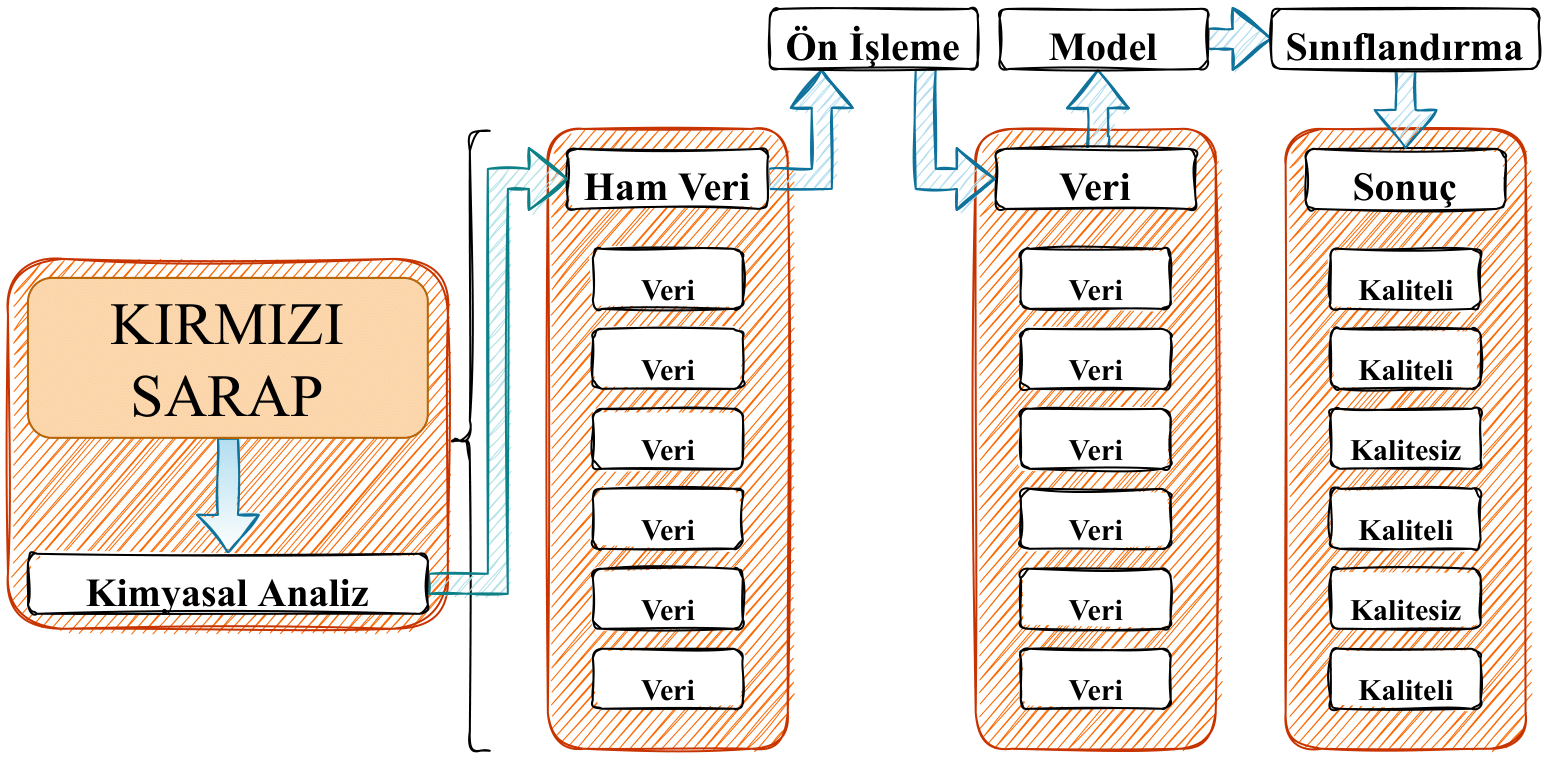
\includegraphics[scale=0.2]{pictures/pic_01.png}&%
		\end{tabular}%
	\end{center}
	\caption{Kırmızı Şarap Kalite Kontrol Süreci}%
	\label{fig:01}
\end{figure}

Projemizin akış diyagramı Şekil \ref{fig:01}'deki gibidir. Makalenin ikinci bölümünde, bahsettiğimiz algortimalar hakkında bilgiler sunulmaktadır. Daha sonraki bölümde ise sonuçlar yer almaktadır.


\section{\textbf{METODLAR}}
\quad Kırmızı şarap kalitesini tahmin edebilmek için belirlediğimiz sınıflandırma algoritmalarını kullandık. Bu algoritmalar aşağıdaki gibidir.
\subsection{\textbf{K-Nearest Neighbor}}
\quad Gözetimli (denetimli) öğrenme metotlarından olup  basit sınıflandırma işlemlerinde kullanılır\cite{8}\cite{9}.Sınıflandırma çalışması yaparken elimizdeki veriler hakkında kısıtlı ön bilgiye sahip olduğumuzda tercih etmemiz gereken ilk algoritmalardan biridir\cite{8}.

\begin{figure}[!h]
	\centering%
	%\scriptsize
	\begin{center}
		\begin{tabular}{cc}%
			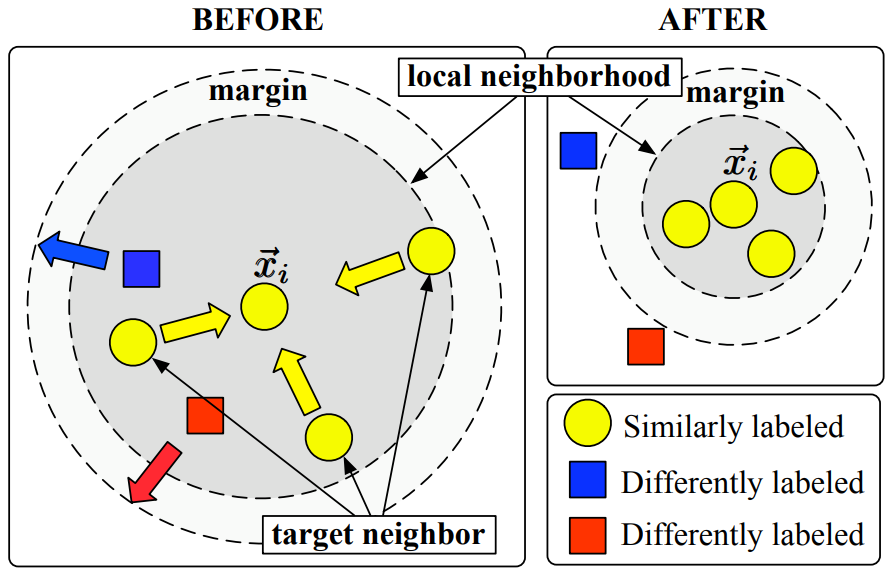
\includegraphics[scale=0.3]{pictures/pic_02.png}&%
		\end{tabular}%
	\end{center}
	\caption{Örnek KNN Şeması\cite{10}}%
	\label{fig:02}
\end{figure}

\quad Bu algoritmanın performansını etkileyen parametreler; uzaklık ölçütü, komşu sayısı(k) ve ağırlıklandırma yöntemidir\cite{7}. Uzaklık ölçütü olarak Manhattan uzaklığı kullandık: \textbf{n} boyutlu düzlemdeki iki konum arasındaki farkların, mutlak değerlerinin toplamıdır. X-Y konumları arasındaki Manhattan uzaklığı: P=(x1, x2,…, xn) ve Q=(y1, y2,…, yn) olmak üzere, Eşitlik \ref{eq:01}'e göre hesaplanır\cite{7}.

\begin{equation}
\label{eq:01}
\Large \sum_{i=1}^{n}\left | x_{i} - y_{i} \right |
\end{equation}

\pagebreak
KNN algoritmasının aşamaları\cite{9}:
\begin{itemize}
\item K değeri belirlenir
\item Diğer konumlara olan uzaklık, Manhattan yöntemiyle hesaplanır
\item Uzaklıklar sıralanarak en yakın komşular bulunur
\item En yakın K adet komşunun kategorileri toplanır
\item Toplam sonucunda ağırlıkta olan kategori seçilerek etiketleme yapılır
\end{itemize}

\subsection{\textbf{Support Vector Machines (SVM)}}
\quad Türkçe adıyla Destek Vektör Makineleri (DVM), istatistiksel öğrenme teorisi geliştiricisi Vapnik tarafından geliştirilmiştir. Sınıflandırma, örüntü tanıma problemleri için kullanılır. Destek Vektör Makineleri, alanındaki birçok tekniğe göre daha yüksek başarı oranına sahiptir. Uygulama sırasında çekirdek fonksiyon seçimi ve parametre optimizasyonu çok önemlidir\cite{11}.

\begin{figure}[!h]
	\centering%
	%\scriptsize
	\begin{center}
		\begin{tabular}{cc}%
			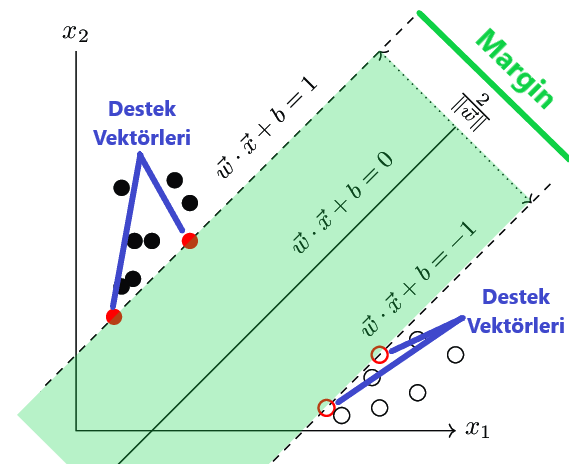
\includegraphics[scale=0.3]{pictures/pic_03.png}&%
		\end{tabular}%
	\end{center}
	\caption{Örnek SVM Şeması\cite{12}}%
	\label{fig:03}
\end{figure}

Şekil \ref{fig:03} üzerinde siyah ve beyaz olmak üzere iki sınıf mevcut. Gelecek verilerin sınıflandırılabilmesi için öncelikle sınıfları birbirinden ayıran bir doğru çizilir. Bu doğrunun -1 ve +1 değerleri arasında kalan yeşil kısım Margin bölgesidir. Margin ne kadar geniş olursa, sınıflar o kadar iyi ayırışıyor demektir. Bu işlemin formülü Eşitlik \ref{eq:02}'deki gibidir.

\begin{equation}
\label{eq:02}
\Large \hat{y}=\left\{\begin{matrix} 0, w^{T} \cdot x + b < 0,\\ 1, w^{T} \cdot x + b \geq 0 \end{matrix}\right.
\end{equation}

\quad Elde ettiğimiz sonuç 0’dan küçük çıkarsa beyaz noktaların bulunduğu kısma yakın olacaktır. Sonuç 0’a eşit veya 0’dan büyük çıkarsa siyah noktaların bulunduğu kısma daha yakın olacaktır\cite{12}.
\pagebreak
\subsection{\textbf{Logistic Regression}}

\quad Lojistik Regresyon,bize sonucu 0 veya 1 şeklinde üreten, değişkenlerin modellenmesinde kullanılan algoritmadır. Örneğin kırmızı şarap kalitesini ele aldığımız zaman; elimizdeki veri setinde 0 kalitesiz, 1 kaliteli durumunu temsil eder. Yani Lojistik Regresyon algoritmasıyla predict edilen verilerin ait oldukları sınıfları tahmin edebiliriz\cite{13}.

\begin{equation}
\label{eq:03}
\Large f(x)=\frac{1}{1+e^{-z}}
\end{equation}

Lojistik regresyon, $\left(-\infty,+\infty \right)$ aralığındaki değerleri girdi olarak kabul eder\cite{13}.

\begin{figure}[!h]
	\centering%
	%\scriptsize
	\begin{center}
		\begin{tabular}{cc}%
			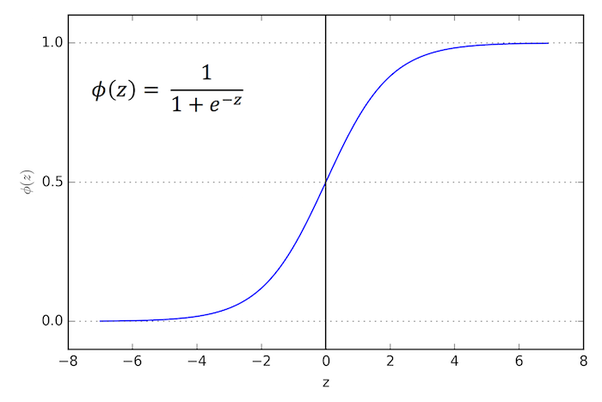
\includegraphics[scale=0.3]{pictures/pic_04.png}&%
		\end{tabular}%
	\end{center}
	\caption{Örnek bir Lojistik Regresyon Şeması\cite{13}}%
	\label{fig:04}
\end{figure}

\subsection{\textbf{Naive Bayes}}
\quad Navie Bayes algoritması sınıflandırıcı teorem olan Bayes’e dayanmaktadır\cite{15}.  Adını ingiliz matematikçi olan Thomas Bayes’ten almıştır\cite{14}. Navie Bayes, elimizdeki örneklerin hangi sınıfa ait olduğunu, işlemler sonucu elde ettiği oranla tahmin eder. Navie Bayes’ın iki önemli kabulü vardır\cite{15}. Bunlar:
\begin{itemize}
\item Elimizde bulunan niteliklerin hepsi aynı derecede önemlidir.
\item Elimizde bulunan nitelikler birbirinden bağımsızdır.
\end{itemize}

\quad Koşullu olasılıklar arasında bağlantı kuran Bayes Teoremi, x özniteliğinin gerçekleşmiş olması durumunda C özniteliğinin gerçekleşmesi veya C özniteliğinin gerçekleşmiş olması durumunda x özniteliğinin gerçekleşmesi durumunu bize verir\cite{15}. Bayes kuralının algoritması Eşitlik \ref{eq:04}'deki gibidir. Eşitlikte yer alan değerler\cite{14}:

\begin{itemize}
\item \textbf{p(x|Cj):} j sınıfından bir örneğin x olma olasılığı
\item \textbf{P(Cj):} j sınıfının ilk olasılığı
\item \textbf{p(x):} Herhangi bir örneğin x olma olasılığı
\item \textbf{P(Cj|x):} x olan bir örneğin j sınıfından olma olasılığı (son olasılık)
\end{itemize}

\begin{equation}
\label{eq:04}
\Large P(C_{j}|x) = \frac {p(x|C_{j}) P(C_{j})} {p(x)} = \frac {p(x|C_{j}) P(C_{j})} {\sum_{k}^{}p(x|C_{k})P(C_{k})}
\end{equation}

\subsection{\textbf{Decision Tree}}
\quad Karar ağaçları, en yaygın kullanılan gözetimli(denetimli) öğrenme algoritmalarından birisidir. Adından da anlaşılacağı üzere ağaç tabanlı öğrenmeye dayalıdır. Tüm problemlere uyarlanabilir\cite{16}. Karar ağacı, kök düğüm değişkeninden başlayarak, ağaç dalı hiyerarşisi gibi dallanır\cite{17}.

\begin{figure}[!h]
	\centering%
	%\scriptsize
	\begin{center}
		\begin{tabular}{cc}%
			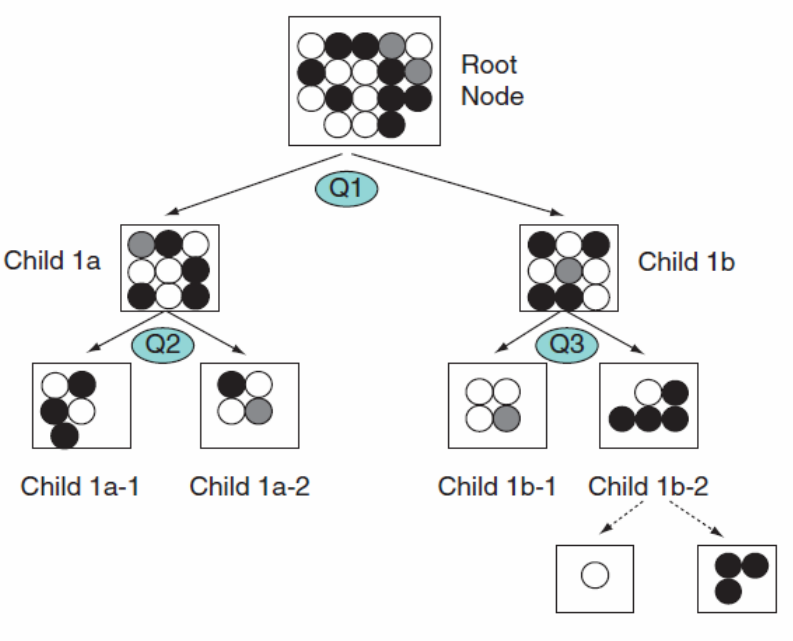
\includegraphics[scale=0.4]{pictures/pic_05.png}&%
		\end{tabular}%
	\end{center}
	\caption{Örnek bir Karar Ağacı Şeması\cite{17}}%
	\label{fig:05}
\end{figure}

\quad Entropi, verilerimizle alakalı belirsizliğin bir ölçüsüdür; dolayısıyla entropinin düşük olması tercih edilir. Verilerimizin tamamı sezgsel olarak aynı etikete sahipse, veri setinin entropisi düşüktür diyebiliriz\cite{16}.

\begin{equation}
\label{eq:05}
\Large H=-\sum p(x)\log{p(x)}
\end{equation}

\quad Burada; p(x) belirli bir sınıfa ait grubun yüzde oranını, H ise entropiyi belirtmektedir. Karar ağacı, entropiyi en aza indirecek şekilde bölünme yapmalıdır. En iyi bölümlemeyi belirlemek için kullanılan bilgi kazancı, Eşitlik \ref{eq:06}'daki gibi hesaplanır\cite{16}.

\begin{equation}
\label{eq:06}
\Large Gain(S,D) = H(S)-\sum_{V\in D}^{}\frac{\left|V\right|}{\left|S\right|}H(V)
\end{equation}

\quad Burada; \textbf{S} orijinal veri kümesini, \textbf{D} ise kümenin bölünmüş bir parçasını temsil eder. Her \textbf{V} değeri, \textbf{S}'nin alt kümesidir\cite{16}.
\pagebreak
\subsection{\textbf{Bagging}}
\quad Türkçe adıyla torbalama yöntemi olarak adlandırılan Bagging algoritması 1996 yılında Breiman tarafından geliştirilmiştir. Bagging (torbalama) algoritmasının çalışma biçimi Şekil \ref{fig:06}'da belirtilmiştir. Şekil \ref{fig:06}'daki aşamaların açıklamaları\cite{18}:

\begin{itemize}
\item \textbf{Bootstrap sampling:} Orijinal veri kümesi, alt kümelere bölünür.
\item \textbf{Model training:} Bu alt kümelerin her birinde ayrı ayrı temel (zayıf) model oluşturulur.
\item \textbf{Model forecasting:} Modeller birbirinden bağımsız ancak paralel olarak çalışır.
\item \textbf{Result aggregating:} Tüm modellerin tahmin sonuçları birleştirilerek niai tahmin belirlenir.
\end{itemize}

\begin{figure}[!h]
	\centering%
	%\scriptsize
	\begin{center}
		\begin{tabular}{cc}%
			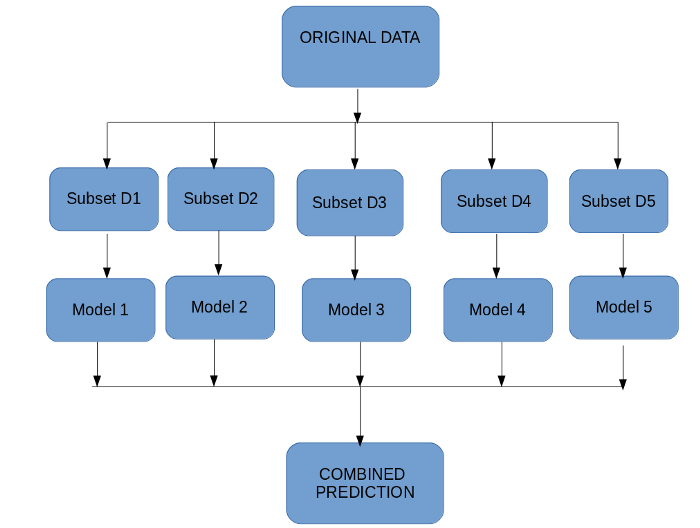
\includegraphics[scale=0.35]{pictures/pic_06.png}&%
		\end{tabular}%
	\end{center}
	\caption{Örnek bir Torbalama Şeması\cite{18}}%
	\label{fig:06}
\end{figure}
\newpage
\subsection{\textbf{Random Forest Tree}}
\quad Türkçe adıyla Rastgele Orman Ağacı Algoritması, denetimli bir sınıflandırma algoritmasıdır. Adından da anlaşılacağı gibi, algoritmamız rastgele bir orman yaratıyor. Ormanda bulubab ağaç sayısı ile elde ettiğimiz çıktılar arasında doğrusal bir ilişki vardır. Ağaç sayısı arttıkça elde edilecek olan sonucun kesinliği de artar. Rastgele Orman Ağacı’nın Karar Ağacı’ndan farkı; kök bulma ve düğümleri bölme işlemlerinin çalışıyor olmasıdır\cite{19}. Rastgele Orman Ağacı’nın şeması Şekil \ref{fig:07}'de verilmiştir.

\begin{figure}[!h]
	\centering%
	%\scriptsize
	\begin{center}
		\begin{tabular}{cc}%
			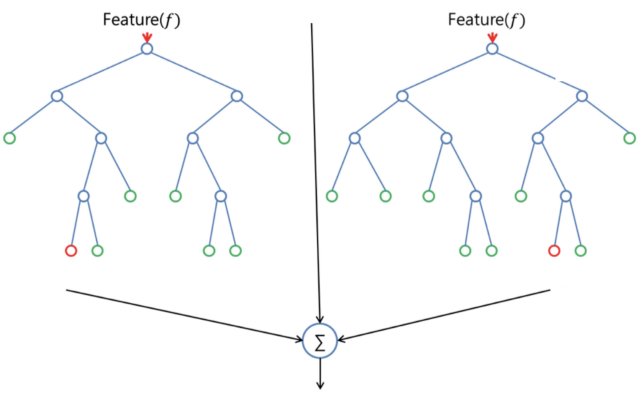
\includegraphics[scale=0.45]{pictures/pic_07.png}&%
		\end{tabular}%
	\end{center}
	\caption{Örnek bir Rastgele Orman Ağacı Şeması\cite{20}}%
	\label{fig:07}
\end{figure}

\quad Rastgele Orman Ağacı, kullanıcıdan iki parametre alır: m parametresi en iyi bölünmeyi belirlemek için her düğümde kullanılan değişkenlerin sayısı, N geliştirilecek ağaç sayısı. Öncelikle eğitim verilerinin 2/3'ü kullanılarak önyükleme örnekleri oluşturulur. Geri kalan 1/3'lük kısım (OOB: out of bag) ise hataları test etmek için kullanılır\cite{21}.

\quad Her bir düğümde \textbf{m} değişkenleri, tüm değişkenlerin arasından rastgele seçilerek en iyi dal belirlenir. \textbf{M} adet değişkenin kareköküne eşit olarak alınan \textbf{m} değişken, genellikle optimuma en yakın sonucu verir\cite{21}.

\quad Sınıfların homojenliği $Gini$ indexi hesaplanarak ölçülür. $Gini$ indexi ne kadar düşükse, sınıf da o kadar homojendir. Bir düğümün alt $Gini$ indexi üst $Gini$ indexinden daha az olduğu durumlarda incelenen dal başarılı sayılır\cite{21}. $Gini$ indexinin formülü Eşitlik \ref{eq:07}'de verilmiştir. Formül değişkenlerinin temsil ettiği veriler de aşağıdaki gibidir;

\begin{itemize}
\item \textbf{T:} Tüm veri seti
\item \textbf{pj:} Veri setindeki her bir verinin kendinden küçük ve kendünden büyük eleman sayılarına bölümü
\item \textbf{n:} Seçilen verimiz
\end{itemize}

\begin{equation}
\label{eq:07}
\Large Gini(T)=1-\sum_{j=1}^{n}(p_{j})^{2}
\end{equation}

\pagebreak
\section{\textbf{SONUÇLAR}}

\quad Elimizdeki veri setinin $\%70$'ini, belirlediğimiz ve açıkladığımız algoritmaların eğitiminde kullandık. Bu eğitimler sonrasında, veri setimizinin geri kalan $\%30$'unu ise predict(tahmin) işlemi için kullanarak algoritma modellerimizi test ettik. Bu testler sonucunda modellerimizin, veri setimiz üzerindeki başarı ve hata oranlarını Şekil \ref{fig:08}'deki grafiğe döktük.

\begin{figure}[!h]
	\centering
	\begin{center}
		\begin{tabular}{cc}
			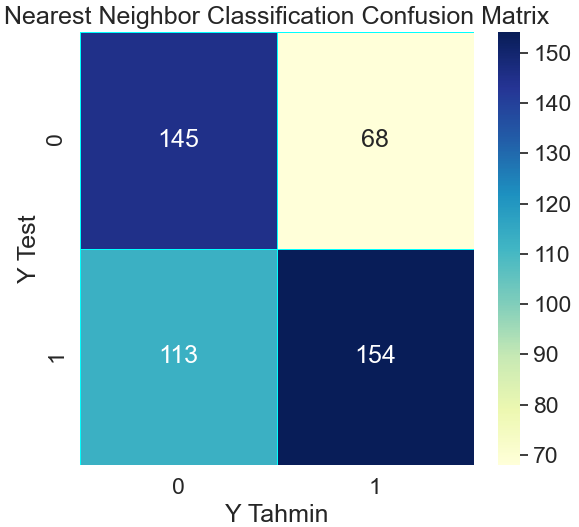
\includegraphics[scale=0.15]{pictures/pic_08.png}&
		\end{tabular}
	\end{center}
	\caption{Tüm Algoritmaların Doğruluk \& MSE Oranları}
	\label{fig:08}
\end{figure}

\quad Kırmızı şarap kalitesinin tahmin edilebilmesi için, "Red Wine Quality"\cite{4} isimli veri seti üzerinden Bagg, DT, KNN, LG, NB, RF ve SVM sınıflandırıcıları kullanılmıştır. Bu algoritmaların $acc$, $MSE$ ve $AUC$ değerleri, Tablo \ref{tbl:01}'de verilmiştir.

\begin{table}[h]
	\centering
	\small
	\begin{tabular}{|l|c|c|c|c|}
		\hline
					& \textbf{acc}	& \textbf{MSE}	& \textbf{AUC}	\\ \hline
		\textbf{Bagg}	& 0.78		& 0.21		& 0.780		\\ \hline
		\textbf{DT}		& 0.76		& 0.23 		& 0.761		\\ \hline
		\textbf{KNN}	& 0.62		& 0.37 		& 0.629		\\ \hline
		\textbf{LG}		& 0.73		& 0.26		& 0.736		\\ \hline
		\textbf{NB}		& 0.74		& 0.25		& 0.743		\\ \hline
		\textbf{RF}		& \textbf{0.80}	& \textbf{0.19}	& \textbf{0.799}	\\ \hline
		\textbf{SVM}	& 0.69		& 0.30		& 0.691		\\ \hline
	\end{tabular}
	\caption{Bagging, DT, KNN, LG, NB, RF ve SVM sınıflandırıcılarının \textit{acc, MSE ve AUC} ölçütlerinin ortalama değerleri}
	\label{tbl:01}
\end{table}

\quad Tablo \ref{tbl:01} incelendiği zaman, en yüksek doğruluk değerine $(acc)$ sahip olan algoritmanın Random Forest $(0.80)$ olduğunu görüyoruz. Ardından bunu takip eden algoritma ise $0.78$ doğruluk oranı ile Bagging Classifier oluyor. Üçüncü sırada ise $0.76$ doğruluk oranıyla Decision Tree algoritması yer alıyor. Geri kalan algoritmaların $acc$ değerleri de Tablo \ref{tbl:01}'de görülmektedir.

\quad $MSE$ (mean squared error/ortalama kare hatası) değerleri için Tablo \ref{tbl:01} incelendiği zaman, en düşük $MSE$ değerine sahip olan algoritmanın Random Forest $(0.19)$ olduğunu görüyoruz. En yüksek $MSE$ değerinin ise $0.37$ oranıyla K-Nearest Neighboor algoritmasına ait olduğunu görüyoruz.

\pagebreak

\subsection{\textbf{Tüm Algoritmalara Ait ROC Eğrisi Grafiği}}

\quad Makine öğrenmesinde performans ölçümünde ROC eğrisinden de yararlanırız. Bu eğrilerin $AUC$(doğruluk) değerleri de mevcuttur ancak algoritmanın tahmin doğruluk skoruyla $(acc)$ karıştırılmamalıdır\cite{22}. Elimizdeki algoritmaların ROC eğrilerini Şekil \ref{fig:09}'da verdik. Eğrilerin doğruluk oranları da Tablo \ref{tbl:01}'de belirtilmiştir.

\begin{figure}[!h]
	\centering
	\begin{center}
		\begin{tabular}{cc}
			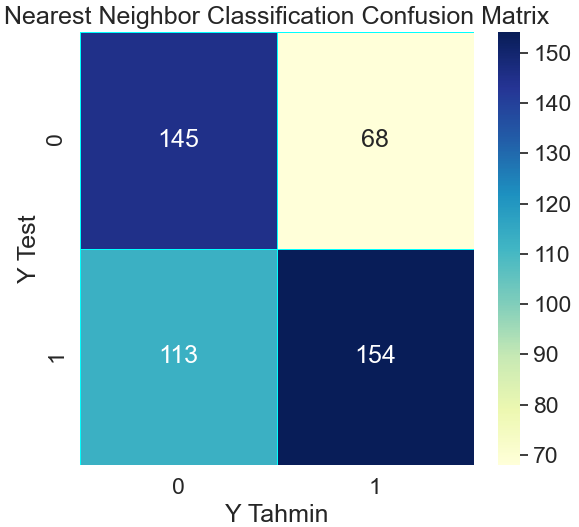
\includegraphics[scale=0.575]{pictures/pic_09.png}&
		\end{tabular}
	\end{center}
	\caption{Tüm Algoritmaların ROC Eğrileri ve AUC Değerleri}
	\label{fig:09}
\end{figure}

\subsection{\textbf{Confusion Matrix (Hata Matrisi)}}

\quad Tablo \ref{tbl:01}'de en yüksek doğruluk $(acc)$ değerine $(0.80)$ sahip olan Random Forest algoritması $0.19$ değeri ile en düşük hata oranına sahiptir. Diğer algoritmalara baktığımız zaman elde edilen doğruluk $(acc)$ ve hata $(MSE)$ değerleri arasında ters orantı vardır. Yani $acc$ değerimiz ne kadar yüksek olursa $MSE$ değerimiz de o kadar düşük olmaktadır.
\begin{itemize}
\item $acc + MSE = 1$
\end{itemize}



\begin{figure}[!h]
	\centering
	\begin{center}
		\begin{tabular}{cc}
			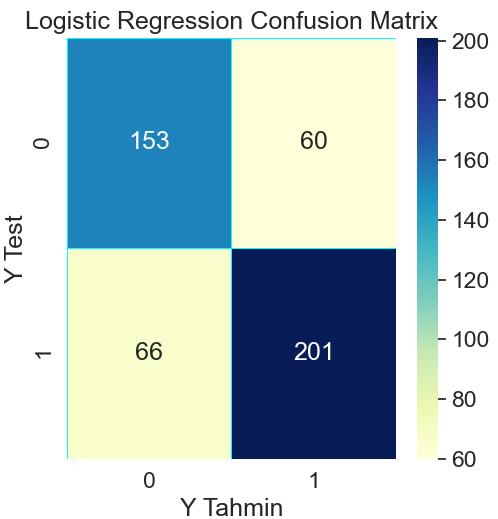
\includegraphics[scale=0.39]{pictures/pic_10.png}&
		\end{tabular}
	\end{center}
	\caption{K-Nearest Neighbor Hata Matrisi}
	\label{fig:10}
\end{figure}
\newpage
\begin{figure}[!h]
	\centering
	\begin{center}
		\begin{tabular}{cc}
			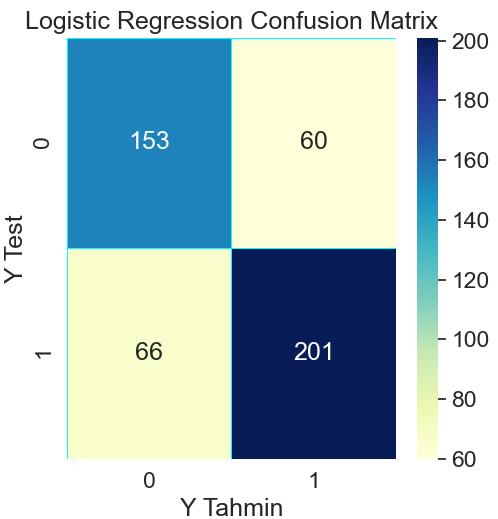
\includegraphics[scale=0.4]{pictures/pic_11.png}&
		\end{tabular}
	\end{center}
	\caption{Support Vector Machines Hata Matrisi}
	\label{fig:11}
\end{figure}

\begin{figure}[!h]
	\centering
	\begin{center}
		\begin{tabular}{cc}
			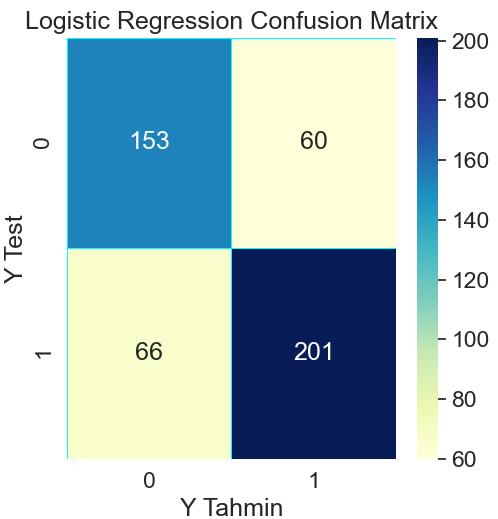
\includegraphics[scale=0.4]{pictures/pic_12.png}&
		\end{tabular}
	\end{center}
	\caption{Logistic Regression Hata Matrisi}
	\label{fig:12}
\end{figure}

\begin{figure}[!h]
	\centering
	\begin{center}
		\begin{tabular}{cc}
			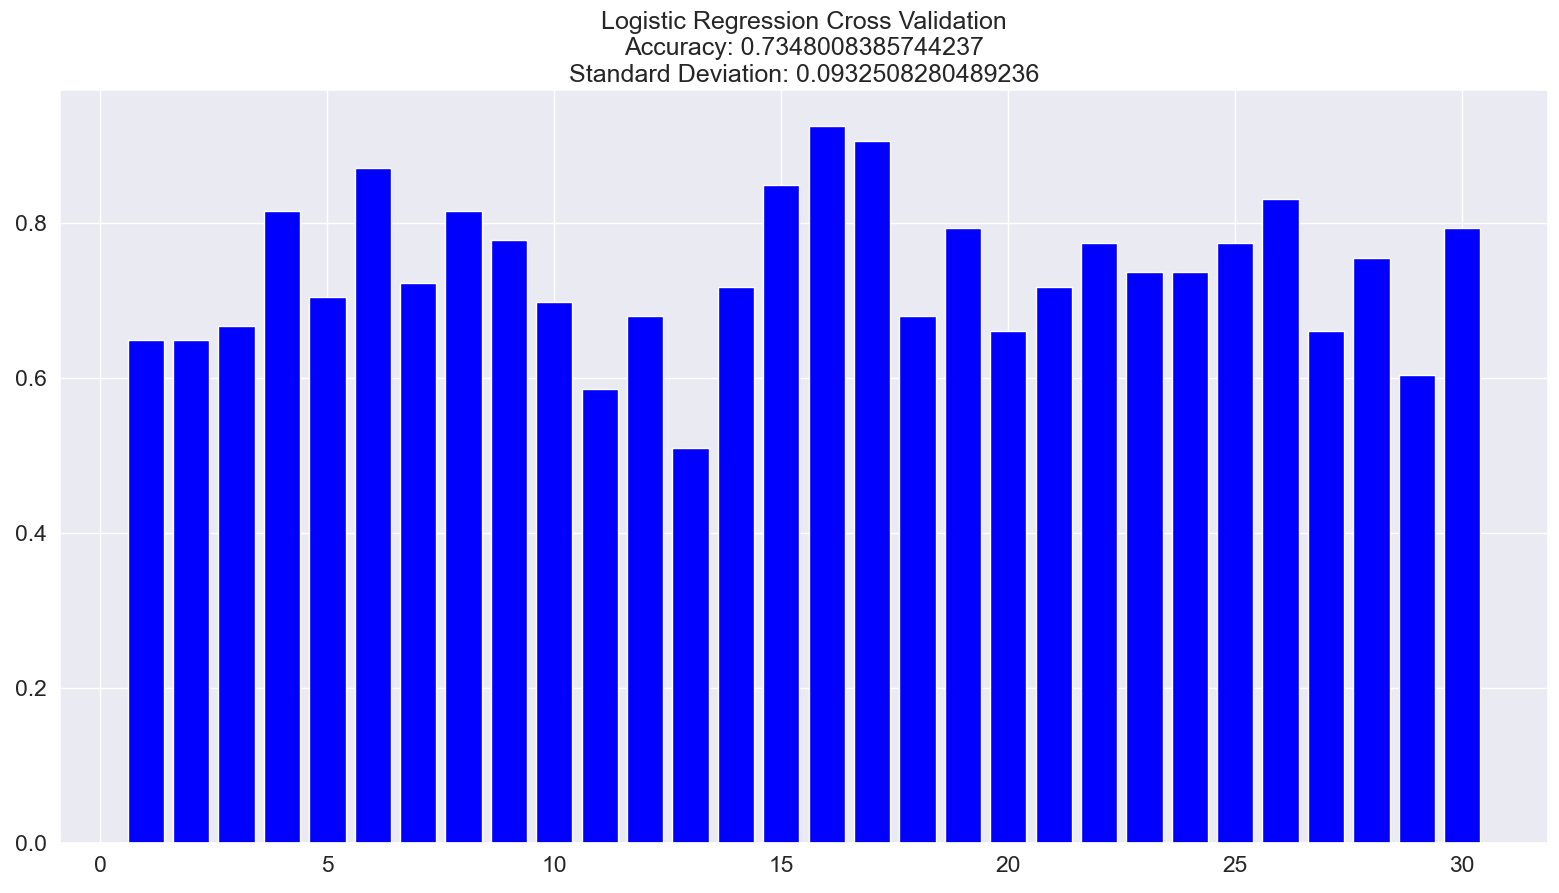
\includegraphics[scale=0.4]{pictures/pic_13.png}&
		\end{tabular}
	\end{center}
	\caption{Naive Bayes Hata Matrisi}
	\label{fig:13}
\end{figure}

\begin{figure}[!h]
	\centering
	\begin{center}
		\begin{tabular}{cc}
			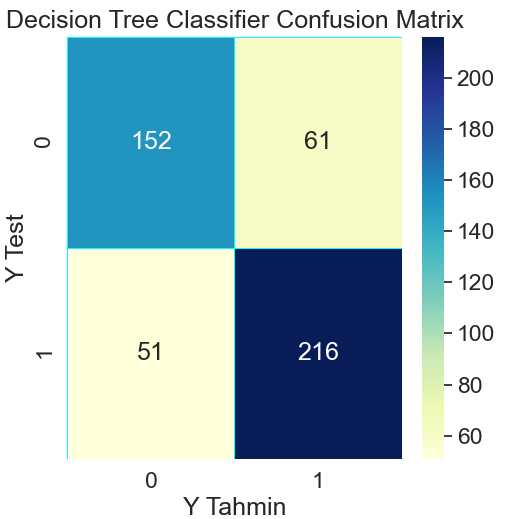
\includegraphics[scale=0.4]{pictures/pic_14.png}&
		\end{tabular}
	\end{center}
	\caption{Decision Tree Hata Matrisi}
	\label{fig:14}
\end{figure}

\begin{figure}[!h]
	\centering
	\begin{center}
		\begin{tabular}{cc}
			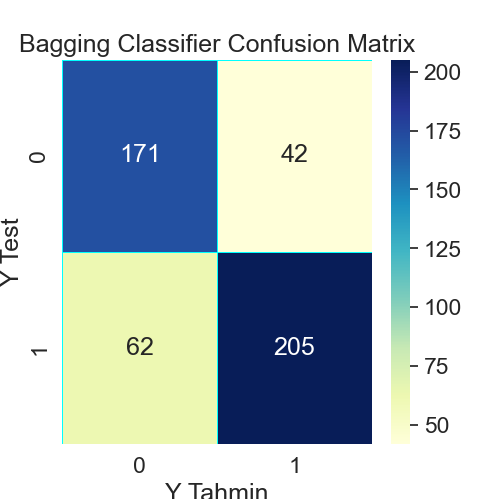
\includegraphics[scale=0.4]{pictures/pic_15.png}&
		\end{tabular}
	\end{center}
	\caption{Bagging Hata Matrisi}
	\label{fig:15}
\end{figure}
\pagebreak
\begin{figure}[!h]
	\centering
	\begin{center}
		\begin{tabular}{cc}
			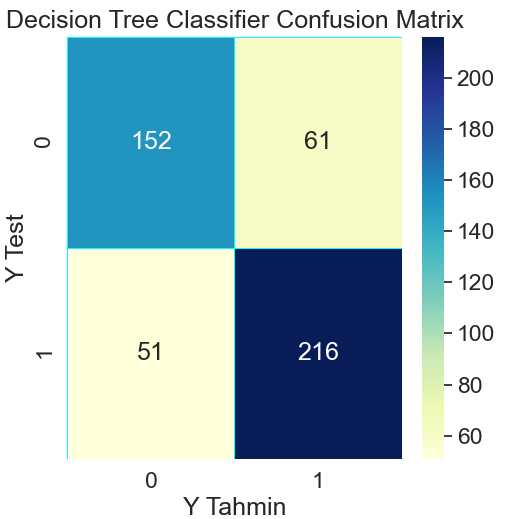
\includegraphics[scale=0.4]{pictures/pic_16.png}&
		\end{tabular}
	\end{center}
	\caption{Random Forest Tree Hata Matrisi}
	\label{fig:16}
\end{figure}
\pagebreak



\newpage
\subsection{\textbf{Cross-Validation (Çapraz Doğrulama)}}
\quad Sınıflandırma algoritmalarımızı bir kez eğittiğimiz zaman elde ettiğimiz verileri Tablo \ref{tbl:01}'de belirttik. Elimizdeki  Bagg, DT, KNN, LG, NB, RF ve SVM algoritmalarının üzerinde, \textbf{10 Kat Çapraz Doğrulama} yöntemini kullanarak 30 farklı koşma işlemi gerçekleştirdik. Bu koşma işlemlerinin tamamı rastgele ve birbirinden bağımsız olduğu için, farklı durumlarda algoritmaların nasıl çalıştığını da daha iyi anlamış olduk.

\begin{figure}[!h]
	\centering
	\begin{center}
		\begin{tabular}{cc}
			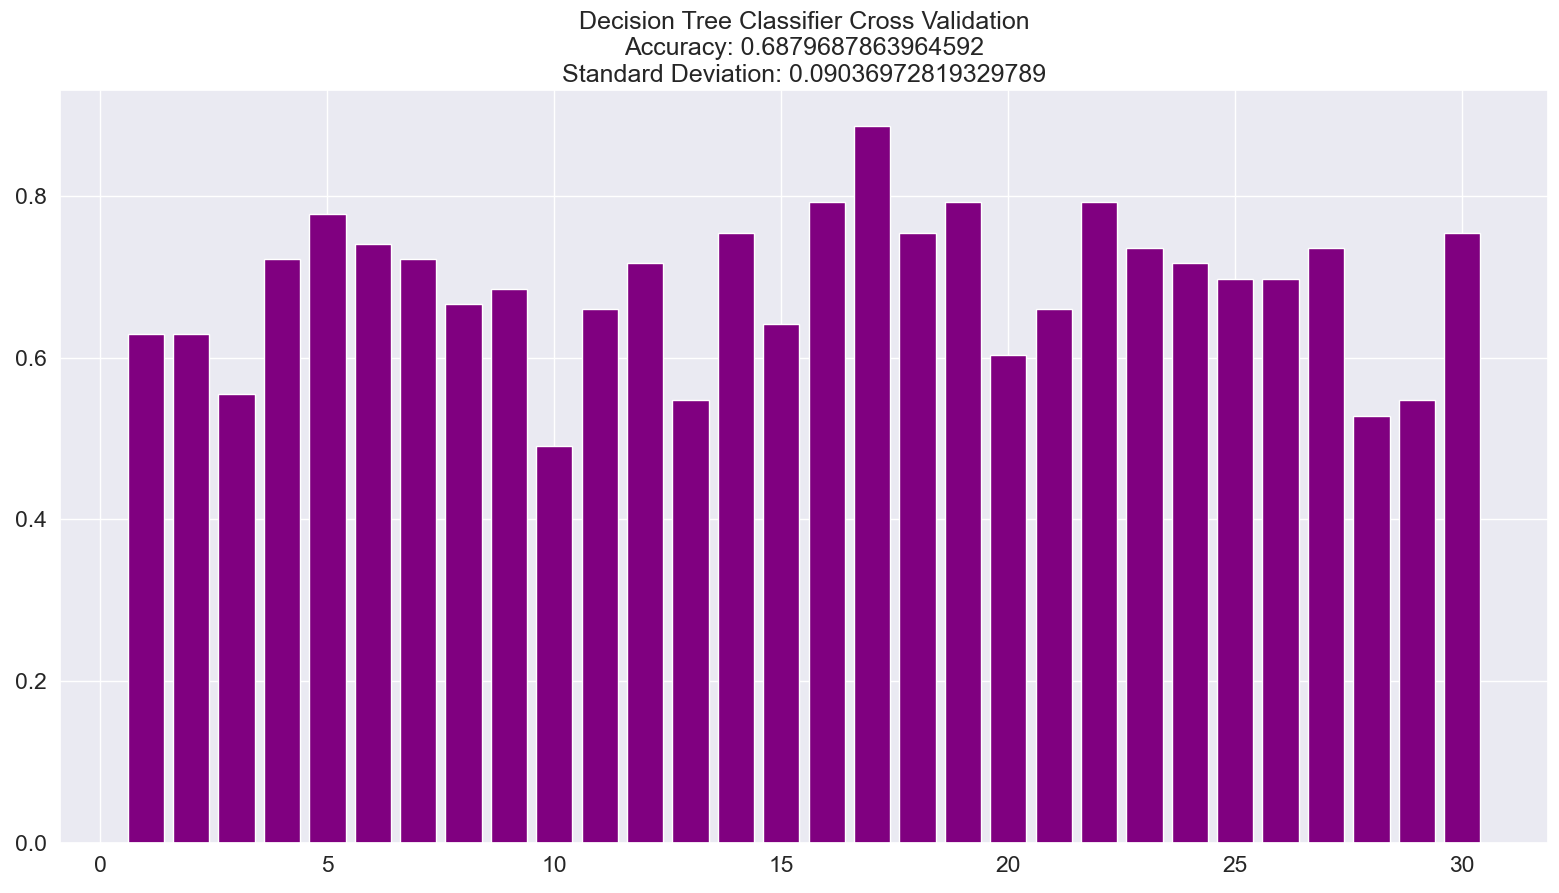
\includegraphics[scale=0.2]{pictures/pic_17.png}&
		\end{tabular}
	\end{center}
	\caption{K-Nearest Neighbor Cross-Validation}
	\label{fig:17}
\end{figure}

\begin{figure}[!h]
	\centering
	\begin{center}
		\begin{tabular}{cc}
			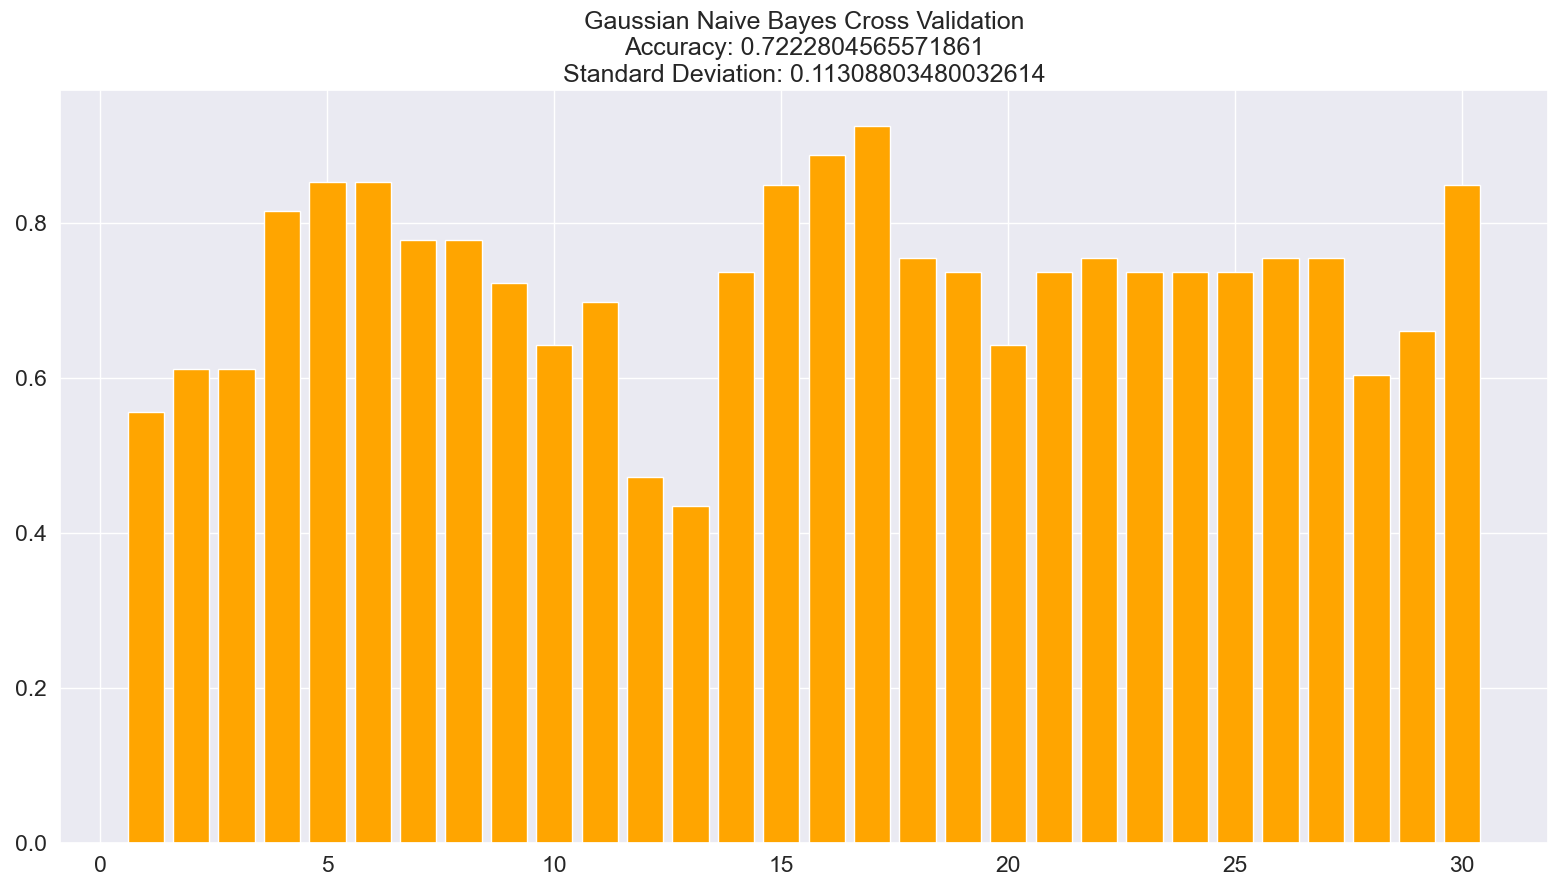
\includegraphics[scale=0.2]{pictures/pic_18.png}&
		\end{tabular}
	\end{center}
	\caption{Support Vector Machines Cross-Validation}
	\label{fig:18}
\end{figure}

\begin{figure}[!h]
	\centering
	\begin{center}
		\begin{tabular}{cc}
			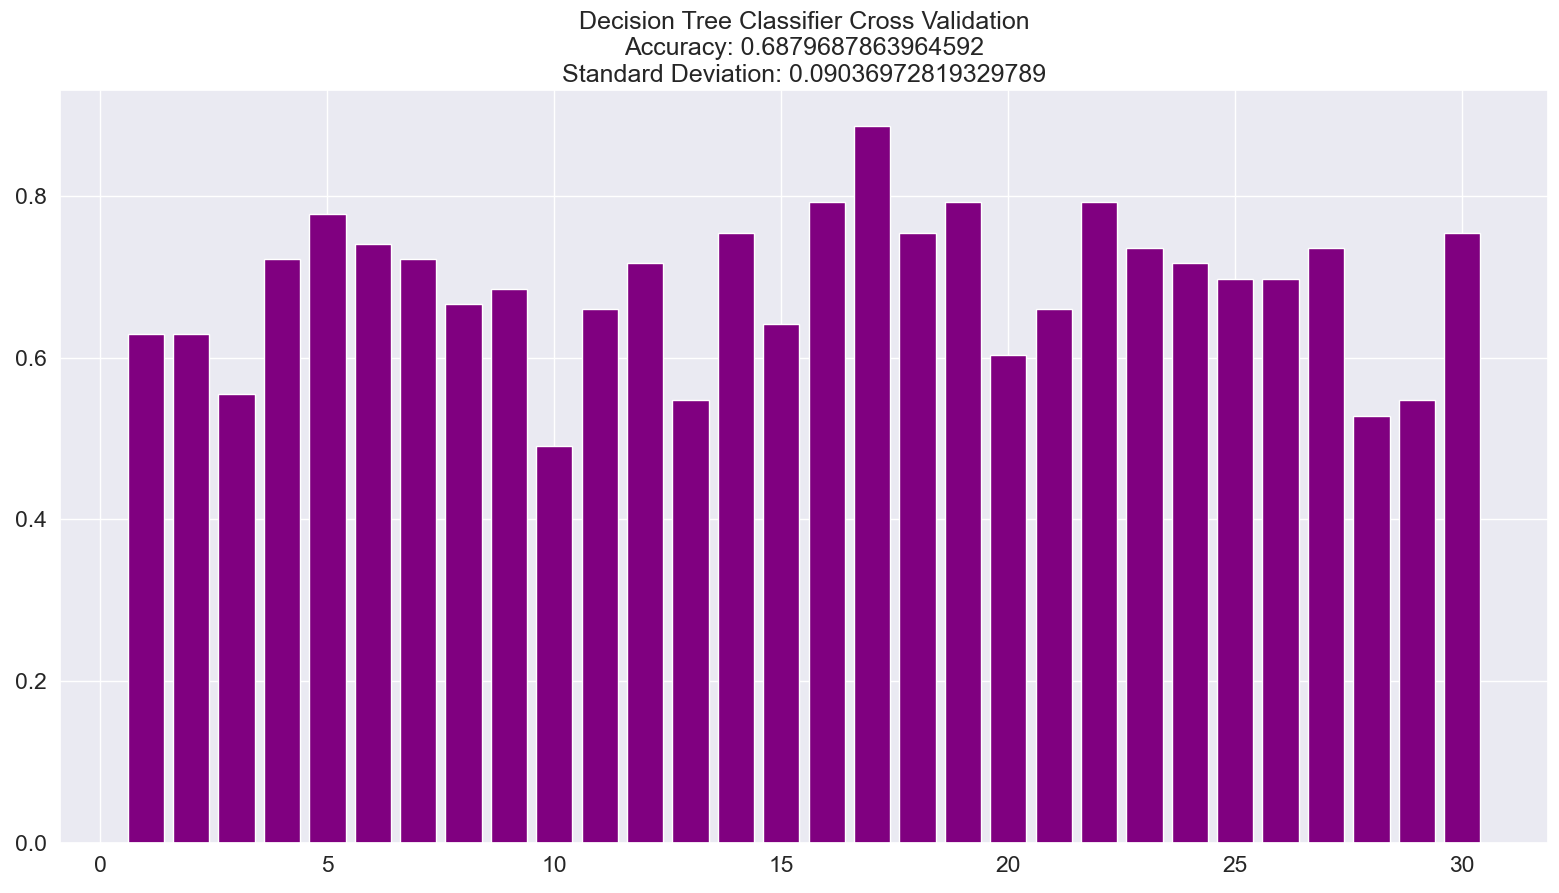
\includegraphics[scale=0.2]{pictures/pic_19.png}&
		\end{tabular}
	\end{center}
	\caption{Logistic Regression Cross-Validation}
	\label{fig:19}
\end{figure}

\begin{figure}[!h]
	\centering
	\begin{center}
		\begin{tabular}{cc}
			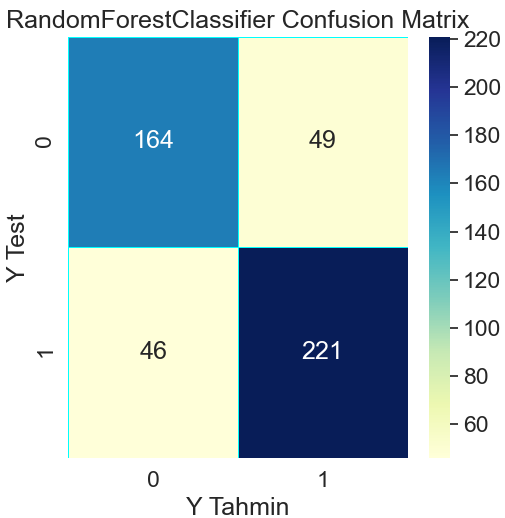
\includegraphics[scale=0.18]{pictures/pic_20.png}&
		\end{tabular}
	\end{center}
	\caption{Naive Bayes Cross-Validation}
	\label{fig:20}
\end{figure}

\begin{figure}[!h]
	\centering
	\begin{center}
		\begin{tabular}{cc}
			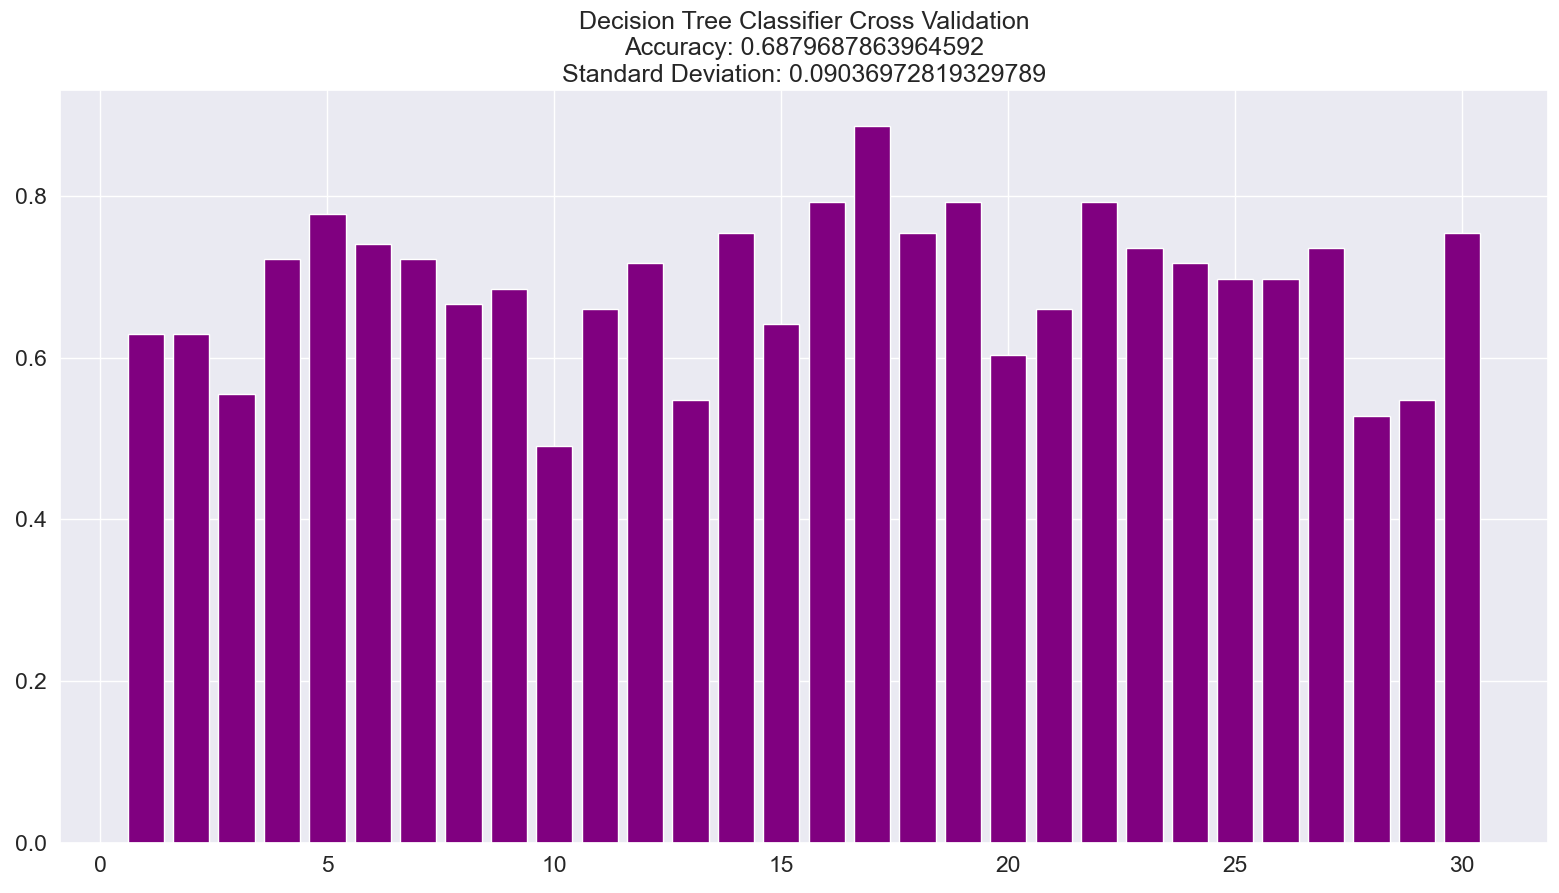
\includegraphics[scale=0.18]{pictures/pic_21.png}&
		\end{tabular}
	\end{center}
	\caption{Decision Tree Cross-Validation}
	\label{fig:21}
\end{figure}

\begin{figure}[!h]
	\centering
	\begin{center}
		\begin{tabular}{cc}
			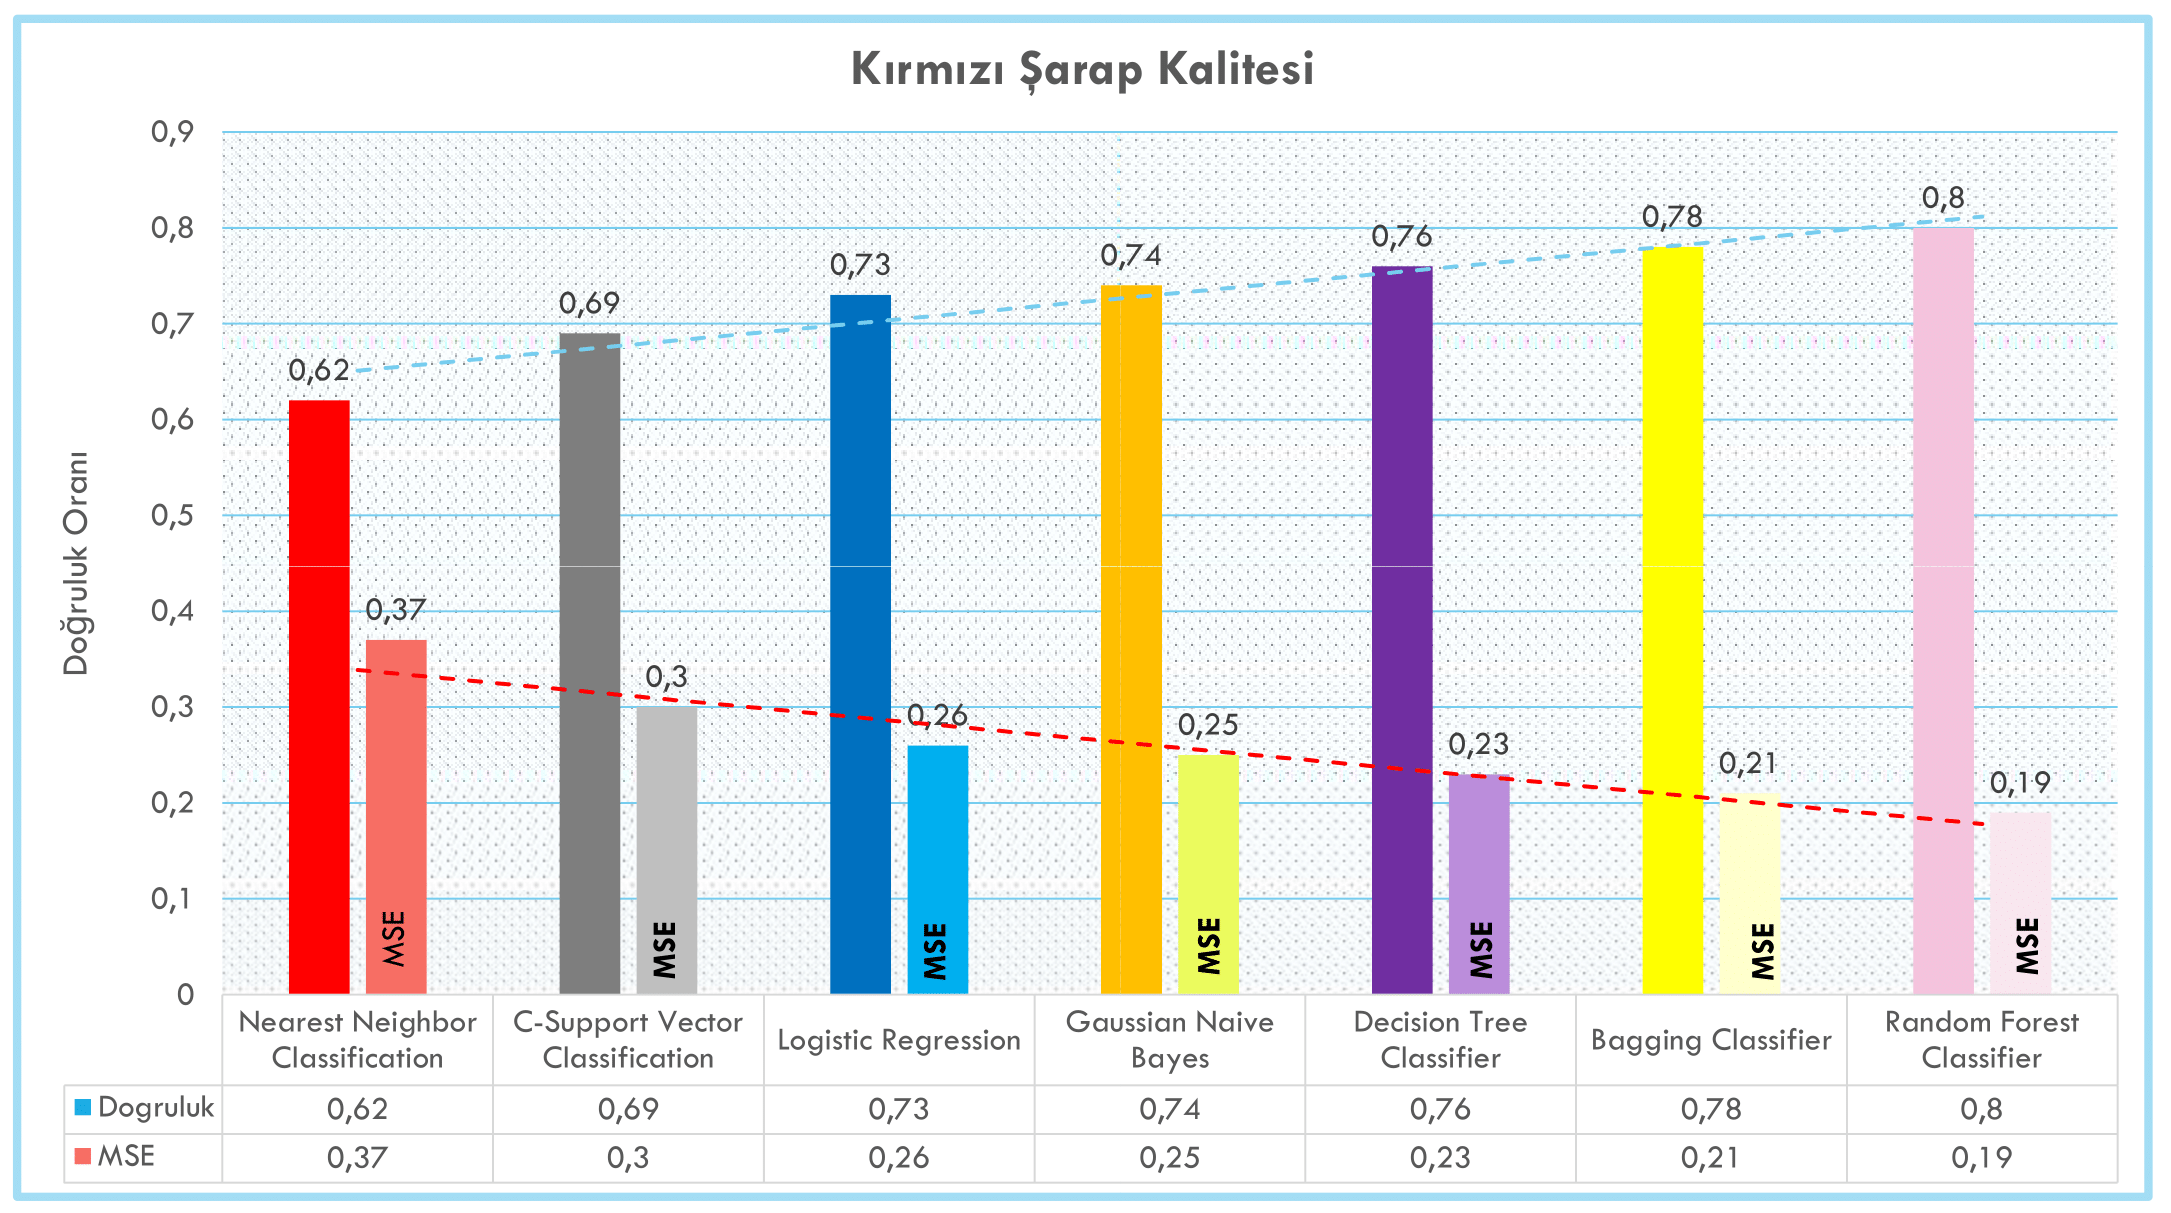
\includegraphics[scale=0.18]{pictures/pic_22.png}&
		\end{tabular}
	\end{center}
	\caption{Bagging Cross-Validation}
	\label{fig:22}
\end{figure}

\begin{figure}[!h]
	\centering
	\begin{center}
		\begin{tabular}{cc}
			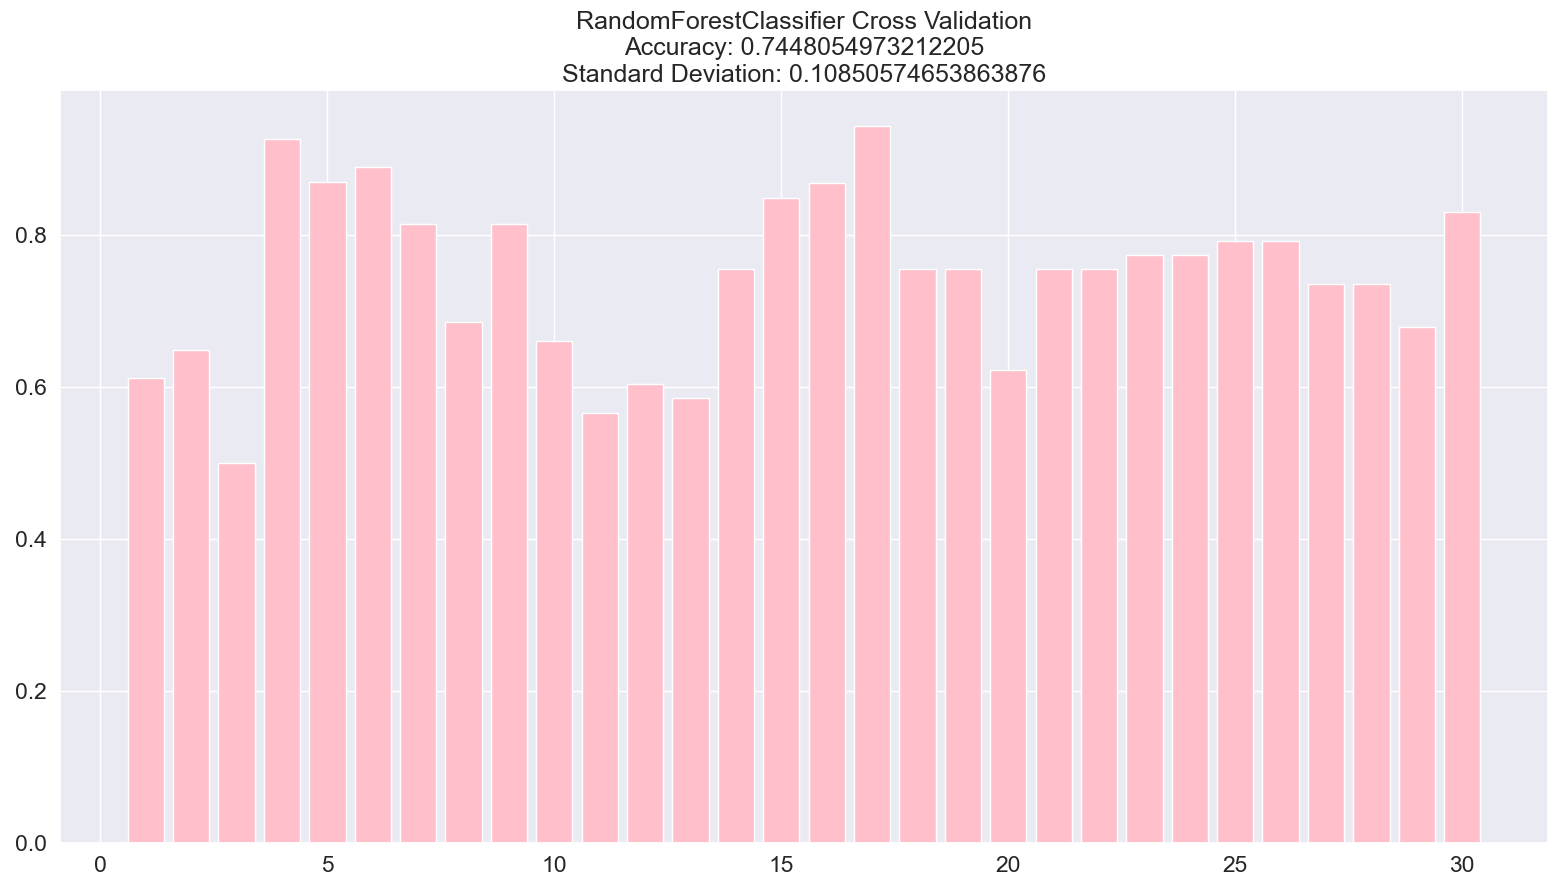
\includegraphics[scale=0.18]{pictures/pic_23.png}&
		\end{tabular}
	\end{center}
	\caption{Random Forest Tree Cross-Validation}
	\label{fig:23}
\end{figure}
\pagebreak

\quad  Bagg, DT, KNN, LG, NB, RF ve SVM algoritmalarını \textbf{10 Kat Çapraz Doğrulama} yöntemi kullanarak eğittik, çıkan sonuçları ise Şekil \ref{fig:17}, \ref{fig:18}, \ref{fig:19}, \ref{fig:20}, \ref{fig:21}, \ref{fig:22} ve \ref{fig:23}'te görselleştirdik. Bu yöntem sonucunda;
\begin{itemize}
\item \textbf{Çalışma Sayısı}$(30) * $\textbf{Algoritma Sayısı}$(7) = \textbf{210}$
\end{itemize}
adet sonuç elde ettik. Bu sonuçların ortalama değerlerini de Tablo \ref{tbl:02}'de belirttik.

\begin{table}[h]
	\centering
	\normalsize
	\begin{tabular}{|l|c|c|c|c|}
		\hline
					& \textbf{acc}	& \textbf{St.Dev.}		\\ \hline
		\textbf{Bagg}	& 0.6986		& 0.0955			\\ \hline
		\textbf{DT}		& 0.6879		& \textbf{0.0903}		\\ \hline
		\textbf{KNN}	& 0.6289		& 0.1050 			\\ \hline
		\textbf{LG}		& 0.7348		& 0.0932			\\ \hline
		\textbf{NB}		& 0.7222		& 0.1130			\\ \hline
		\textbf{RF}		& \textbf{0.7448}	& 0.1085			\\ \hline
		\textbf{SVM}	& 0.7179		& 0.1032			\\ \hline
	\end{tabular}
	\caption{Bagging, DT, KNN, LG, NB, RF ve SVM sınıflandırıcılarının \textbf{Cross-Validation (10 Kat Çapraz Doğrulama)} sonuçlarının ortalama değerleri}
	\label{tbl:02}
\end{table}

\quad Tablo \ref{tbl:02}'deki değerlere baktığımız zaman en yüksek doğruluk ortalamasına sahip algoritmanın Random Forest $(0.7448)$ ve en düşük standart devinasyon ortalamasına sahip algoritmanın da Decision Tree $(0.0903)$ olduğunu görüyoruz.

\quad Logistic Regression algoritmasının $acc$ değerlerine baktığımız zaman diğer algoritmaların ortalamasının üstünde kaldığını ve $StandardDevination$ değerinin de diğer algoritmaların ortalamasının altında kaldığını görüyoruz. Bu senaryoda en verimli algoritmalardan birinin de Logistic Regression olduğunu söyleyebiliriz.

%%%%%%%%%%%%%%%%%%%%

\newpage
\section{\textbf{SONUÇ}}
\quad Bu projede kullanılan veri seti sayesinde kırmızı şarabın kalitesinin, ortalamanın üstünde veya altında olduğunu tahmin etmeye çalıştık. Bunu yapmak için, önceden belirlediğimiz algoritmaları kullandık ve sonuçlarını karşılaştırdık. Her algoritmada farklı doğruluk değerleri elde ettik. Bazı algoritmalar bu veri seti için daha yeterli olurken bazıları daha yetersiz kaldı. Algoritmaların veri setiyle verimli çalışabilmesi için, veri setinin detaylandırılması gerekir. Bunu da doğru özniteliklerin eklenmesi veya çıkartılması, örnek sayısının çoğaltılmasıyla sağlayabiliriz. Bu sayede kalite ölçümünü daha efektif hale getirebiliriz.

\begin{figure}[!h]
	\centering
	\begin{center}
		\begin{tabular}{cc}
			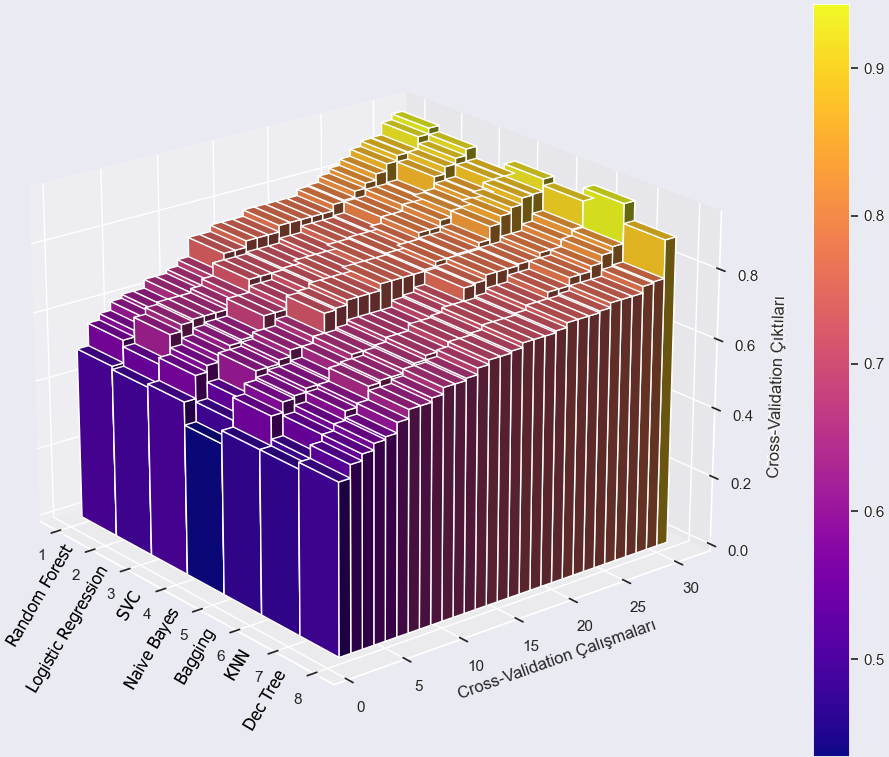
\includegraphics[scale=0.35]{pictures/pic_24.png}&
		\end{tabular}
	\end{center}
	\caption{Tüm Algoritmaların Cross-Validation Sonuçlarının 3D Grafiği}
	\label{fig:24}
\end{figure}

\quad $X-ekseni$'ne baktığımız zaman algoritmalarımızın isimlerini, $Y-ekseni$'ne baktığımızda ise bu algoritmaların çalışma sayılarını görüyoruz. Elimizdeki $X-Y$ şeklindeki 2D ortama 3. bir boyut ekleyerek, bu algoritmaların çalışma sonuçlarını da $Z-ekseni$'ne eklemiş oluyoruz.

\quad Elimizdeki bu 3D grafiği incelersek, en yüksek ortalamaya sahip algoritmanın Random Forest olduğunu anlayabiliriz. Çalışma sonuçlarını küçükten büyüğe sıralayarak bir rampa oluşmasını sağladık. Bu sayede rampanın yüksek kısmında kalan algoritmalar yüksek verimliliğer sahip algoritmalar oldu.

%%%%%%%%%%%%%%%%%%%%
\newpage
\begin{thebibliography}{6}

\bibitem{1} 
DergiPark - Şarap Üretimi ve Kalite
\\\texttt{\href{https://dergipark.org.tr/tr/download/article-file/498270}{\nolinkurl{dergipark.org.tr/sarap-uretimi-ve-kalite}}}

\bibitem{2} 
Wikipedia - Şarap
\\\texttt{\href{https://tr.wikipedia.org/wiki/Şarap}{\nolinkurl{wikipedia.org/Şarap}}}

\bibitem{3} 
Resmi Gazete - Türk Gıda Kodeksi Şarap Tebliği
\\\texttt{\href{https://www.resmigazete.gov.tr/eskiler/2009/02/20090204-12.htm}{\nolinkurl{resmigazete.gov.tr/2009/02/20090204-12}}}

\bibitem{4} 
Kaggle - Red Wine Quality Dataset
\\\texttt{\href{https://www.kaggle.com/uciml/red-wine-quality-cortez-et-al-2009}{\nolinkurl{kaggle.com/red-wine-quality}}}

\bibitem{5} 
Wine Quality Exploration
\\\texttt{\href{http://rstudio-pubs-static.s3.amazonaws.com/80458_5000e31f84df449099a872ccf40747b7.html}{\nolinkurl{amazonaws.com/wine-quality-exploration}}}

\bibitem{6} 
Hydrometer Confusion
\\\texttt{\href{http://www.creativeconnoisseur.com/newsletter/files/497deafe6be1b2efc87df8ac6071e459-162.html}{\nolinkurl{creativeconnoisseur.com/hydrometer-confusion}}}

\bibitem{7} 
Erdal Taşçı \& Aytuğ Onan - KNN Algorithm
\\\texttt{\href{https://ab.org.tr/ab16/bildiri/102.pdf}{\nolinkurl{ab.org.tr/knn-algorithm}}}

\bibitem{8} 
Scholarpedia - K-Nearest Neighbor
\\\texttt{\href{http://scholarpedia.org/article/K-nearest_neighbor}{\nolinkurl{scholarpedia.org/K-nearest_neighbor}}}

\bibitem{9} 
Erdinç Uzun - KNN Algoritması
\\\texttt{\href{https://erdincuzun.com/makine_ogrenmesi/k-nn-algoritmasi/}{\nolinkurl{erdincuzun.com/makine_ogrenmesi/k-nn-algoritmasi}}}

\bibitem{10} 
Large Margin Nearest Neighbor Classification
\\\texttt{\href{https://proceedings.neurips.cc/paper/2005/file/a7f592cef8b130a6967a90617db5681b-Paper.pdf}{\nolinkurl{proceedings.neurips.cc/Margin_Nearest_Neighbor_Classification.pdf}}}

\bibitem{11} 
DergiPark - Destek Vektör Makinesi
\\\texttt{\href{https://dergipark.org.tr/tr/download/article-file/65371}{\nolinkurl{dergipark.org.tr/Destek_Vektor_Makinesi}}}

\bibitem{12} 
Medium - Destek Vektör Makineleri
\\\texttt{\href{https://medium.com/deep-learning-turkiye/nedir-bu-destek-vektör-makineleri-makine-öğrenmesi-serisi-2-94e576e4223e}{\nolinkurl{medium.com/deep-learning-turkiye/destek-vektör-makineleri}}}

\bibitem{13} 
Medium - Lojistik Regresyon
\\\texttt{\href{https://medium.com/@k.ulgen90/lojistik-regresyon-makine-öğrenimi-bölüm-7-c6bc685a4084}{\nolinkurl{medium.com/lojistik-regresyon-makine-öğrenimi}}}

\bibitem{14} 
Başken Üniversitesi - Naive Bayes
\\\texttt{\href{https://mail.baskent.edu.tr/~20410964/DM_9.pdf}{\nolinkurl{baskent.edu.tr/Naive_Bayes.pdf}}}

\bibitem{15} 
Akademik Bilişim - Naive Bayes
\\\texttt{\href{https://ab.org.tr/ab14/bildiri/186.pdf}{\nolinkurl{ab.org.tr/Naive_Bayes.pdf}}}

\bibitem{16} 
Medium - Karar Ağaçları
\\\texttt{\href{https://medium.com/@k.ulgen90/makine-öğrenimi-bölüm-5-karar-ağaçları-c90bd7593010}{\nolinkurl{medium.com/makine-öğrenimi-karar-ağaçları}}}

\bibitem{17} 
Sosyal Araştırmalar - Karar Ağacı
\\\texttt{\href{https://www.sosyalarastirmalar.com/articles/text-classification-via-decision-trees-algorithm-customer-comments-case.pdf}{\nolinkurl{sosyalarastirmalar.com/decision-trees-algorithm}}}

\bibitem{18} 
Medium - Ensemble Learning
\\\texttt{\href{https://medium.com/deep-learning-turkiye/ensemble-learning-bagging-ve-boosting-50643428b22b}{\nolinkurl{medium.com/ensemble-learning-bagging-ve-boosting}}}

\bibitem{19} 
Medium - Rastgele Orman Ağacı Algoritması
\\\texttt{\href{https://medium.com/@cemthecebi/rastgele-orman-algoritması-1600ca4f4784}{\nolinkurl{medium.com/rastgele-orman-algoritması}}}

\bibitem{20} 
DevHunter - Rastgele Orman Ağacı Algoritması
\\\texttt{\href{https://devhunteryz.wordpress.com/2018/09/20/rastgele-ormanrandom-forest-algoritmasi/comment-page-1}{\nolinkurl{devhunteryz.com/rastgele-ormanrandom-forest-algoritmasi}}}

\bibitem{21} 
SlideShare - Rastgele Orman Ağacı Algoritması
\\\texttt{\href{https://www.slideshare.net/SezerFidanc/random-forest-algoritmas}{\nolinkurl{slideshare.net/random-forest-algoritması}}}

\bibitem{22} 
Medium - ROC Eğrisi
\\\texttt{\href{https://bernatas.medium.com/roc-eğrisi-ve-eğri-altında-kalan-alan-auc-97b058e8e0cf}{\nolinkurl{medium.com/roc-eğrisi}}}


\end{thebibliography}

\end{document}
